% Options for packages loaded elsewhere
\PassOptionsToPackage{unicode}{hyperref}
\PassOptionsToPackage{hyphens}{url}
\documentclass[
  catalan,
  a4paper,
]{article}
\usepackage{xcolor}
\usepackage[margin=1in]{geometry}
\usepackage{amsmath,amssymb}
\setcounter{secnumdepth}{-\maxdimen} % remove section numbering
\usepackage{iftex}
\ifPDFTeX
  \usepackage[T1]{fontenc}
  \usepackage[utf8]{inputenc}
  \usepackage{textcomp} % provide euro and other symbols
\else % if luatex or xetex
  \usepackage{unicode-math} % this also loads fontspec
  \defaultfontfeatures{Scale=MatchLowercase}
  \defaultfontfeatures[\rmfamily]{Ligatures=TeX,Scale=1}
\fi
\usepackage{lmodern}
\ifPDFTeX\else
  % xetex/luatex font selection
\fi
% Use upquote if available, for straight quotes in verbatim environments
\IfFileExists{upquote.sty}{\usepackage{upquote}}{}
\IfFileExists{microtype.sty}{% use microtype if available
  \usepackage[]{microtype}
  \UseMicrotypeSet[protrusion]{basicmath} % disable protrusion for tt fonts
}{}
\usepackage{setspace}
\makeatletter
\@ifundefined{KOMAClassName}{% if non-KOMA class
  \IfFileExists{parskip.sty}{%
    \usepackage{parskip}
  }{% else
    \setlength{\parindent}{0pt}
    \setlength{\parskip}{6pt plus 2pt minus 1pt}}
}{% if KOMA class
  \KOMAoptions{parskip=half}}
\makeatother
\usepackage{color}
\usepackage{fancyvrb}
\newcommand{\VerbBar}{|}
\newcommand{\VERB}{\Verb[commandchars=\\\{\}]}
\DefineVerbatimEnvironment{Highlighting}{Verbatim}{commandchars=\\\{\}}
% Add ',fontsize=\small' for more characters per line
\usepackage{framed}
\definecolor{shadecolor}{RGB}{248,248,248}
\newenvironment{Shaded}{\begin{snugshade}}{\end{snugshade}}
\newcommand{\AlertTok}[1]{\textcolor[rgb]{0.94,0.16,0.16}{#1}}
\newcommand{\AnnotationTok}[1]{\textcolor[rgb]{0.56,0.35,0.01}{\textbf{\textit{#1}}}}
\newcommand{\AttributeTok}[1]{\textcolor[rgb]{0.13,0.29,0.53}{#1}}
\newcommand{\BaseNTok}[1]{\textcolor[rgb]{0.00,0.00,0.81}{#1}}
\newcommand{\BuiltInTok}[1]{#1}
\newcommand{\CharTok}[1]{\textcolor[rgb]{0.31,0.60,0.02}{#1}}
\newcommand{\CommentTok}[1]{\textcolor[rgb]{0.56,0.35,0.01}{\textit{#1}}}
\newcommand{\CommentVarTok}[1]{\textcolor[rgb]{0.56,0.35,0.01}{\textbf{\textit{#1}}}}
\newcommand{\ConstantTok}[1]{\textcolor[rgb]{0.56,0.35,0.01}{#1}}
\newcommand{\ControlFlowTok}[1]{\textcolor[rgb]{0.13,0.29,0.53}{\textbf{#1}}}
\newcommand{\DataTypeTok}[1]{\textcolor[rgb]{0.13,0.29,0.53}{#1}}
\newcommand{\DecValTok}[1]{\textcolor[rgb]{0.00,0.00,0.81}{#1}}
\newcommand{\DocumentationTok}[1]{\textcolor[rgb]{0.56,0.35,0.01}{\textbf{\textit{#1}}}}
\newcommand{\ErrorTok}[1]{\textcolor[rgb]{0.64,0.00,0.00}{\textbf{#1}}}
\newcommand{\ExtensionTok}[1]{#1}
\newcommand{\FloatTok}[1]{\textcolor[rgb]{0.00,0.00,0.81}{#1}}
\newcommand{\FunctionTok}[1]{\textcolor[rgb]{0.13,0.29,0.53}{\textbf{#1}}}
\newcommand{\ImportTok}[1]{#1}
\newcommand{\InformationTok}[1]{\textcolor[rgb]{0.56,0.35,0.01}{\textbf{\textit{#1}}}}
\newcommand{\KeywordTok}[1]{\textcolor[rgb]{0.13,0.29,0.53}{\textbf{#1}}}
\newcommand{\NormalTok}[1]{#1}
\newcommand{\OperatorTok}[1]{\textcolor[rgb]{0.81,0.36,0.00}{\textbf{#1}}}
\newcommand{\OtherTok}[1]{\textcolor[rgb]{0.56,0.35,0.01}{#1}}
\newcommand{\PreprocessorTok}[1]{\textcolor[rgb]{0.56,0.35,0.01}{\textit{#1}}}
\newcommand{\RegionMarkerTok}[1]{#1}
\newcommand{\SpecialCharTok}[1]{\textcolor[rgb]{0.81,0.36,0.00}{\textbf{#1}}}
\newcommand{\SpecialStringTok}[1]{\textcolor[rgb]{0.31,0.60,0.02}{#1}}
\newcommand{\StringTok}[1]{\textcolor[rgb]{0.31,0.60,0.02}{#1}}
\newcommand{\VariableTok}[1]{\textcolor[rgb]{0.00,0.00,0.00}{#1}}
\newcommand{\VerbatimStringTok}[1]{\textcolor[rgb]{0.31,0.60,0.02}{#1}}
\newcommand{\WarningTok}[1]{\textcolor[rgb]{0.56,0.35,0.01}{\textbf{\textit{#1}}}}
\usepackage{longtable,booktabs,array}
\usepackage{calc} % for calculating minipage widths
% Correct order of tables after \paragraph or \subparagraph
\usepackage{etoolbox}
\makeatletter
\patchcmd\longtable{\par}{\if@noskipsec\mbox{}\fi\par}{}{}
\makeatother
% Allow footnotes in longtable head/foot
\IfFileExists{footnotehyper.sty}{\usepackage{footnotehyper}}{\usepackage{footnote}}
\makesavenoteenv{longtable}
\usepackage{graphicx}
\makeatletter
\newsavebox\pandoc@box
\newcommand*\pandocbounded[1]{% scales image to fit in text height/width
  \sbox\pandoc@box{#1}%
  \Gscale@div\@tempa{\textheight}{\dimexpr\ht\pandoc@box+\dp\pandoc@box\relax}%
  \Gscale@div\@tempb{\linewidth}{\wd\pandoc@box}%
  \ifdim\@tempb\p@<\@tempa\p@\let\@tempa\@tempb\fi% select the smaller of both
  \ifdim\@tempa\p@<\p@\scalebox{\@tempa}{\usebox\pandoc@box}%
  \else\usebox{\pandoc@box}%
  \fi%
}
% Set default figure placement to htbp
\def\fps@figure{htbp}
\makeatother
\ifLuaTeX
\usepackage[bidi=basic]{babel}
\else
\usepackage[bidi=default]{babel}
\fi
% get rid of language-specific shorthands (see #6817):
\let\LanguageShortHands\languageshorthands
\def\languageshorthands#1{}
\setlength{\emergencystretch}{3em} % prevent overfull lines
\providecommand{\tightlist}{%
  \setlength{\itemsep}{0pt}\setlength{\parskip}{0pt}}
\usepackage{bookmark}
\IfFileExists{xurl.sty}{\usepackage{xurl}}{} % add URL line breaks if available
\urlstyle{same}
\hypersetup{
  pdftitle={U5. UBUNTU. ESTRUCTURA},
  pdfauthor={@tofermos 2026},
  pdflang={ca-ES},
  hidelinks,
  pdfcreator={LaTeX via pandoc}}

\title{U5. UBUNTU. ESTRUCTURA}
\author{@tofermos 2026}
\date{}

\begin{document}
\maketitle

{
\setcounter{tocdepth}{2}
\tableofcontents
}
\setstretch{1.5}
\newpage
\renewcommand\tablename{Tabla}

\section{1. El Sistema Operatiu GNU/Linux. Estructura i
característiques}\label{el-sistema-operatiu-gnulinux.-estructura-i-caracteruxedstiques}

\subsection{1.1 El sistema operatiu
GNU/Linux}\label{el-sistema-operatiu-gnulinux}

\begin{itemize}
\tightlist
\item
  \textbf{GNU/Linux} és un sistema operatiu lliure i de codi obert.
\item
  Basat en el nucli \textbf{Linux} i eines del projecte \textbf{GNU}.
\item
  Escalable: pot ser utilitzat en dispositius menuts o grans servidors.
\end{itemize}

\subsection{1.2 Estructura}\label{estructura}

\begin{enumerate}
\def\labelenumi{\arabic{enumi}.}
\tightlist
\item
  \textbf{Nucli (Kernel)}:

  \begin{itemize}
  \item
    Gestió de recursos: memòria, CPU, dispositius.
  \item
    Per veure la versió:

\begin{Shaded}
\begin{Highlighting}[]
\FunctionTok{uname} \AttributeTok{{-}r}
\end{Highlighting}
\end{Shaded}
  \item
    Exemple de resultat: \texttt{6.8.0-149-generic}
  \end{itemize}
\item
  \textbf{Shell}:

  \begin{itemize}
  \tightlist
  \item
    Interfície que permet interactuar amb el sistema.
  \item
    Exemples: \textbf{bash}, \textbf{sh}, \textbf{dash}.
  \end{itemize}
\end{enumerate}

Els shells disponibles els tenim al fitxer \emph{/etc/shells}

\begin{Shaded}
\begin{Highlighting}[]
\FunctionTok{cat}\NormalTok{ /etc/shells}
\end{Highlighting}
\end{Shaded}

\begin{enumerate}
\def\labelenumi{\arabic{enumi}.}
\setcounter{enumi}{2}
\tightlist
\item
  \textbf{Utilitats}:

  \begin{itemize}
  \tightlist
  \item
    Comandes bàsiques: \texttt{ls}, \texttt{cp}, \texttt{mv}.
  \end{itemize}
\item
  \textbf{Aplicacions}:

  \begin{itemize}
  \tightlist
  \item
    Programes per a usuaris finals, com navegadors, editors; usuaris
    administradors com net-tools, apt o usuaris programadors com
    Visual-Studio
  \end{itemize}
\item
  \textbf{Sistema d'arxius}:

  \begin{itemize}
  \tightlist
  \item
    Estructura jeràrquica que comença a \texttt{/}.
  \end{itemize}
\end{enumerate}

\section{1.3 Característiques}\label{caracteruxedstiques}

\begin{itemize}
\tightlist
\item
  \textbf{Lliure i obert}: Es pot modificar i distribuir.
\item
  \textbf{Multiusuari}: Diversos usuaris alhora.
\item
  \textbf{Multitasca}: Execució de múltiples processos.
\item
  \textbf{Segur}: Model de permisos.
\item
  \textbf{Portabilitat}: Funciona en diferents plataformes.
\end{itemize}

\section{2. Evolució històrica}\label{evoluciuxf3-histuxf2rica}

\begin{itemize}
\tightlist
\item
  \textbf{1991}: Linus Torvalds crea el nucli Linux.
\item
  \textbf{1992}: Es llança com a programari lliure.
\item
  \textbf{1994}: Primera versió estable (Linux 1.0).
\item
  \textbf{Actualitat}: Moltes distribucions basades en Linux.
\end{itemize}

\section{3. Distribucions i versions}\label{distribucions-i-versions}

\begin{itemize}
\tightlist
\item
  Una distribució és una combinació del nucli, utilitats GNU, i altres
  programes.
\end{itemize}

\textbf{Exemples de distribucions:}

\begin{longtable}[]{@{}ll@{}}
\toprule\noalign{}
\textbf{Distribució} & \textbf{Orientació} \\
\midrule\noalign{}
\endhead
\bottomrule\noalign{}
\endlastfoot
Ubuntu & Usuaris nous, suport comunitari. \\
Debian & Estable, molt usada en servidors. \\
Arch Linux & Personalitzable, usuaris experts. \\
\end{longtable}

\textbf{Versió d'Ubuntu i de kernel}

\begin{longtable}[]{@{}
  >{\raggedright\arraybackslash}p{(\linewidth - 2\tabcolsep) * \real{0.5000}}
  >{\raggedright\arraybackslash}p{(\linewidth - 2\tabcolsep) * \real{0.5000}}@{}}
\toprule\noalign{}
\begin{minipage}[b]{\linewidth}\raggedright
Ordre
\end{minipage} & \begin{minipage}[b]{\linewidth}\raggedright
Què mostra
\end{minipage} \\
\midrule\noalign{}
\endhead
\bottomrule\noalign{}
\endlastfoot
\texttt{uname\ -r} & Versió del nucli Linux (kernel). \\
\texttt{uname\ -a} & Informació del nucli, arquitectura i nom de
l'equip. \\
\texttt{lsb\_release\ -a} & Distribució, versió i nom en clau del
sistema operatiu. \\
\texttt{lsb\_release\ -d} & Descripció de la distribució. \\
\texttt{cat\ /etc/os-release} & Informació de la distribució sense
necessitar \texttt{lsb\_release}. \\
\end{longtable}

Una vegada més veiem com en un fitxer de text pla es guarda informació
del sistema. En este cas:

Si lsb-release no està instal·lat, podeu instal·lar-lo:

\begin{verbatim}
sudo apt install lsb-release
\end{verbatim}

\section{4. ENTORN GRÀFIC.}\label{entorn-gruxe0fic.}

\subsection{4.1 Capes o components}\label{capes-o-components}

\begin{figure}
\centering
\pandocbounded{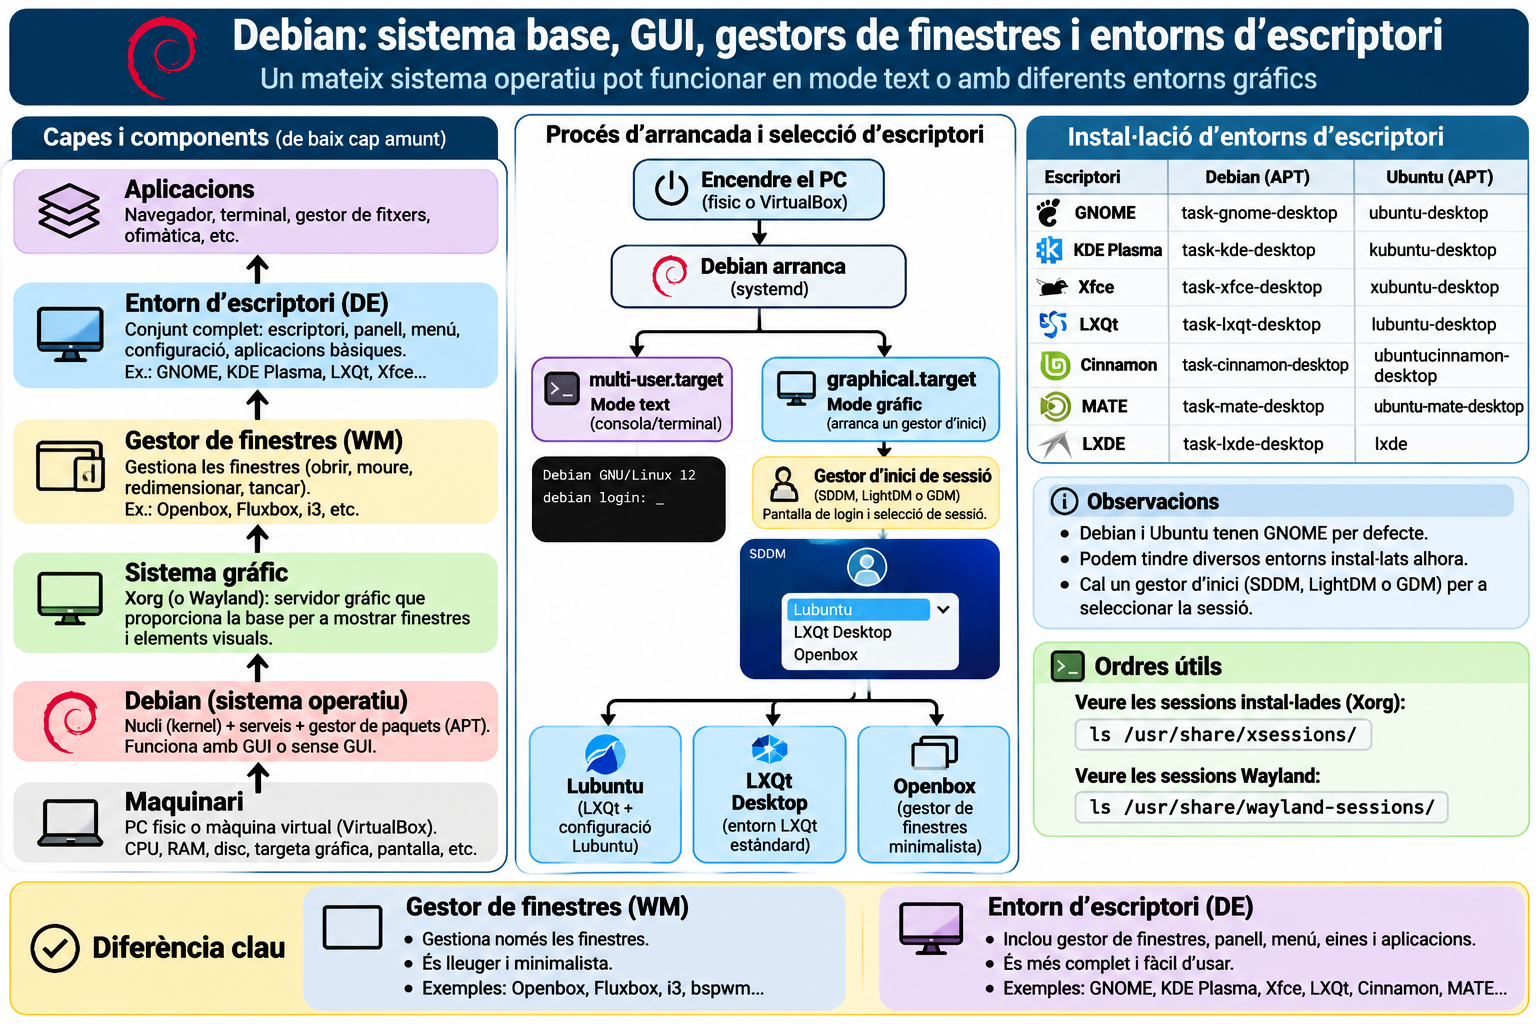
\includegraphics[keepaspectratio]{png/GUI.png}}
\caption{Capes GUI}
\end{figure}

\subsection{4.2 Sistema gràfic i Gestor de
finestres}\label{sistema-gruxe0fic-i-gestor-de-finestres}

\textbf{Sistema gràfic (xorg)}

Com infraestructura per crear entorn gràfic (sistema gràfic) usem
**xorg* Per inicar-lo des del CLI usem el paquet \textbf{xinti} que ens
proporciona el \textbf{startx}

\begin{verbatim}
startx /usr/bin/openbox-session
\end{verbatim}

En el tema de Debian has vist com automatizar-ho en el .xinitrc

\subsubsection{Gestor de finestres}\label{gestor-de-finestres}

\begin{longtable}[]{@{}
  >{\raggedright\arraybackslash}p{(\linewidth - 2\tabcolsep) * \real{0.4444}}
  >{\raggedright\arraybackslash}p{(\linewidth - 2\tabcolsep) * \real{0.5556}}@{}}
\toprule\noalign{}
\begin{minipage}[b]{\linewidth}\raggedright
\textbf{Gestor de finestres}
\end{minipage} & \begin{minipage}[b]{\linewidth}\raggedright
Instal·lar: Sistema gràfic + Gestor de finestres + startx
\end{minipage} \\
\midrule\noalign{}
\endhead
\bottomrule\noalign{}
\endlastfoot
Openbox & \texttt{sudo\ apt\ install\ xorg\ openbox\ xinit} \\
IceWM & \texttt{sudo\ apt\ install\ xorg\ xinit\ icewn} \\
Fluxbox & \texttt{sudo\ apt\ install\ xorg\ xinit\ fluxbox} \\
i3 & \texttt{sudo\ apt\ install\ xorg\ xinit\ i3-wm} \\
\end{longtable}

\subsection{4.3 Escriptoris}\label{escriptoris}

A diferència de Windows, el Linux en tenim més d'un i, a més, en una
mateixa màquina podem tindre'n instal·lat més dun i escollir en iniciar.

\subsubsection{Instal·lació
d'escriptoris}\label{installaciuxf3-descriptoris}

Pots instal·lar escriptoris alternatius en Ubuntu utilitzant el gestor
de paquets \textbf{apt}. Després d'instal·lar-los, pots seleccionar quin
entorn utilitzar en la pantalla d'inici de sessió.

\begin{longtable}[]{@{}
  >{\raggedright\arraybackslash}p{(\linewidth - 4\tabcolsep) * \real{0.3333}}
  >{\raggedright\arraybackslash}p{(\linewidth - 4\tabcolsep) * \real{0.3333}}
  >{\raggedright\arraybackslash}p{(\linewidth - 4\tabcolsep) * \real{0.3333}}@{}}
\toprule\noalign{}
\begin{minipage}[b]{\linewidth}\raggedright
Escriptori
\end{minipage} & \begin{minipage}[b]{\linewidth}\raggedright
Debian
\end{minipage} & \begin{minipage}[b]{\linewidth}\raggedright
Ubuntu
\end{minipage} \\
\midrule\noalign{}
\endhead
\bottomrule\noalign{}
\endlastfoot
\textbf{GNOME} & \texttt{sudo\ apt\ install\ task-gnome-desktop} &
\texttt{sudo\ apt\ install\ ubuntu-desktop} \\
\textbf{LXQt} & \texttt{sudo\ apt\ install\ task-lxqt-desktop} &
\texttt{sudo\ apt\ install\ lubuntu-desktop} \\
\textbf{Xfce} & \texttt{sudo\ apt\ install\ task-xfce-desktop} &
\texttt{sudo\ apt\ install\ xubuntu-desktop} \\
\textbf{KDE Plasma} & \texttt{sudo\ apt\ install\ task-kde-desktop} &
\texttt{sudo\ apt\ install\ kubuntu-desktop} \\
\textbf{Cinnamon} & \texttt{sudo\ apt\ install\ task-cinnamon-desktop} &
\texttt{sudo\ apt\ install\ ubuntucinnamon-desktop} \\
\textbf{MATE} & \texttt{sudo\ apt\ install\ task-mate-desktop} &
\texttt{sudo\ apt\ install\ ubuntu-mate-desktop} \\
\textbf{LXDE} & \texttt{sudo\ apt\ install\ task-lxde-desktop} &
\texttt{sudo\ apt\ install\ lxde-desktop} \\
\end{longtable}

\subsubsection{Com cnsultar els que tenim
instal·lats?}\label{com-cnsultar-els-que-tenim-installats}

Si estem usant la infraestructura gràfica Xorg

\begin{verbatim}
ls /usr/share/xsessions/
\end{verbatim}

Si usarem la infraestructura Wayland

\texttt{ls\ /usr/share/wayland-sessions/}

Per saber quin escriptori estem usant:

\begin{verbatim}
echo $DG_CURRENT_DESKTOP
\end{verbatim}

o també

\texttt{echo\ \$DESKTOP\_SESSION}

\subsection{5.4 Configurar Gestor
d'inici.}\label{configurar-gestor-dinici.}

Com hem dit podem tindre més d'un escriptori instal·lat al PC. El
\textbf{Gestor d'inici} és el software que ens permet triar amb quin
Esciptori iniciar.

Per saber si ja en tenim un instal·lat:

\begin{verbatim}
cat /etc/X11/default-display-manager
\end{verbatim}

Si no en tenim cap instal·lat cal fer-ho ( instal·lem el \emph{sddm})

\begin{verbatim}
sudo apt update
sudo apt install sddm
\end{verbatim}

o un altre (el \emph{LigthDM})

\begin{verbatim}
sudo update
sudo apt install LightDM
\end{verbatim}

Si hem instal·lat els dos, hem d'inicar quin s'iniciarà per defecte:

\begin{verbatim}
sudo dpkg-reconfigure sddm
\end{verbatim}

Imatge del sddm
\pandocbounded{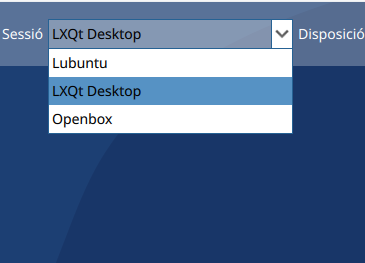
\includegraphics[keepaspectratio]{png/sddm.png}}

\subsection{5.5 Arrencar amb i sense
GUI}\label{arrencar-amb-i-sense-gui}

Si volem iniciar sense GUI, podem configurar-ho i reiniciar (reboot)

\begin{verbatim}
sudo systemctl set-default multi-user.target
sudo reboot
\end{verbatim}

Per inicar amb el GUI, farem l'equivalent:

\begin{verbatim}
sudo systemctl set-graphical.target
sudo reboot
\end{verbatim}

\subsubsection{5.7 Desinstal·lació
d'escriptoris}\label{desinstallaciuxf3-descriptoris}

Per desinstal·lar un escriptori, elimina els paquets associats.
Assegura't de no eliminar dependències crítiques del sistema.

\textbf{Exemple}

\begin{Shaded}
\begin{Highlighting}[]
   \FunctionTok{sudo}\NormalTok{ apt remove task{-}gnome{-}desktop}
   \FunctionTok{sudo}\NormalTok{ apt autoremove}
\end{Highlighting}
\end{Shaded}

\textbf{Si és el Escriptori en ús (o l'últim que queda), has d'iniciar
prèviament sense GUI com hem vist}

\subsection{5.8 Exploradors de fitxers}\label{exploradors-de-fitxers}

Un explorador de fitxers és l'eina gràfica que permet navegar pel
sistema d'arxius. Cada entorn gràfic sol utilitzar un explorador que té
associat però podem instal·lar altres, desinstal·lar i canviar.

\begin{longtable}[]{@{}
  >{\raggedright\arraybackslash}p{(\linewidth - 6\tabcolsep) * \real{0.1301}}
  >{\raggedright\arraybackslash}p{(\linewidth - 6\tabcolsep) * \real{0.1789}}
  >{\raggedright\arraybackslash}p{(\linewidth - 6\tabcolsep) * \real{0.3415}}
  >{\raggedright\arraybackslash}p{(\linewidth - 6\tabcolsep) * \real{0.3496}}@{}}
\toprule\noalign{}
\begin{minipage}[b]{\linewidth}\raggedright
\textbf{Explorador}
\end{minipage} & \begin{minipage}[b]{\linewidth}\raggedright
\textbf{Entorn associat}
\end{minipage} & \begin{minipage}[b]{\linewidth}\raggedright
\textbf{Característiques}
\end{minipage} & \begin{minipage}[b]{\linewidth}\raggedright
\textbf{Com instal·lar-lo}
\end{minipage} \\
\midrule\noalign{}
\endhead
\bottomrule\noalign{}
\endlastfoot
\textbf{Nautilus} & GNOME & Senzill i integrat amb GNOME. &
\texttt{sudo\ apt\ install\ nautilus} \\
\textbf{Thunar} & Xfce & Lleuger i ràpid. &
\texttt{sudo\ apt\ install\ thunar} \\
\textbf{Dolphin} & KDE & Altament personalitzable i complet. &
\texttt{sudo\ apt\ install\ dolphin} \\
\textbf{Caja} & MATE & Similar a Nautilus, però amb opcions clàssiques.
& \texttt{sudo\ apt\ install\ caja} \\
\textbf{PCManFM} & LXDE & Lleuger i senzill. &
\texttt{sudo\ apt\ install\ pcmanfm} \\
\end{longtable}

\subsubsection{Desinstal·lació
d'exploradors}\label{desinstallaciuxf3-dexploradors}

Per exemple, per eliminar \textbf{Caja}:

\begin{Shaded}
\begin{Highlighting}[]
\FunctionTok{sudo}\NormalTok{ apt remove caja}
\FunctionTok{sudo}\NormalTok{ apt autoremove}
\end{Highlighting}
\end{Shaded}


\end{document}
